% !TEX root=../presentation_1.tex
\section{Background}

\subsection{Basic Assumptions}

\begin{frame}
\frametitle{Basic Assumptions}
\begin{itemize}
\item Synchronous CONGEST model.
\begin{itemize}
    \item \textbf{Synchronous} message-passing model.
    \item Every message is $O(\log n)$ in length.
\end{itemize}
\item Every vertex $v$ knows its own \textbf{unique} ID.
\item MST is \textbf{unique}
\begin{itemize}
    \item We can always break the symmetry by encode the weights with fractions to be a function of node ID.
\end{itemize}
\end{itemize}
\end{frame}

\subsection{Summary of methods}
\begin{frame}
\frametitle{Summary of methods}

\begin{itemize}
    \item $n=|V|, m=|E|.$
    \item $D:$ Hop-diameter of the graph. $D=\max_{u,v \in V} dist(u, v)$.
\end{itemize}
% !TEX root=../presentation_1.tex
\begin{table}
\renewcommand{\arraystretch}{1.3}
\caption{Summary of the complexity of distributed MST algorithms}
\begin{tabular}{|c|c|c|}
\hline
Method         & Time Complexity            & Message Complexity\\
\hline
\hline
Pipeline-MST   & $O(D + n)$                 & $O(m + n^2)$\\
\hline
GHS            & $O(n \log n)$              & $O(m + n \log n)$\\
\hline
Controlled-GHS & $O(D + \sqrt{n} \log^* n)$ & $O(m + n^{\frac{3}{2}})$\\
\hline
\textbf{This Work}& $O((D + \sqrt{n}) \log n)$  & $O(m \log n + n \log n \log^* n)$ \\
\hline
\hline
Randomized [PRS16]& $\tilde{O}(D + \sqrt{n})$  & $\tilde{O}(m)$ \\
\hline
Lower Bound [PRS16] & $\tilde{\Omega}(D + \sqrt{n})$  & $\Omega(m)$ \\
\hline
\end{tabular}
\end{table}

\end{frame}

\subsection{Pipeline-MST}
\begin{frame}
\frametitle{Pipeline-MST}
\begin{itemize}
    \item A distributed version of \textbf{Kruskal's} algorithm.
    \item Build a BFS tree first, $O(D)$ rounds with $O(m)$ messages.
    \item Each node keeps a candidate set, initializes at neighbor edges.
    \item For each round
    \begin{itemize}
        \item Add the incoming edges to the set.
        \item Remove the \textbf{heaviest} edge in any \textbf{cycle} in the set.
        \item Send the \textbf{lightest} candidate to its BFS parent.
    \end{itemize}
\end{itemize}
\end{frame}

\begin{frame}
\frametitle{Pipeline-MST}
\begin{itemize}
    \item $O(D+n)$ rounds:
    \begin{itemize}
        \item $O(D)$ rounds to reach from the leaves to the root.
        \item $O(n)$ rounds to find the edges needed for an MST.
    \end{itemize}
    \item $O(m)$ messages to build BFS tree. Each node sends $O(n)$ edges.
    \item $O(D+n)$ rounds and $O(m + n^2)$ messages.
\end{itemize}
\begin{figure}
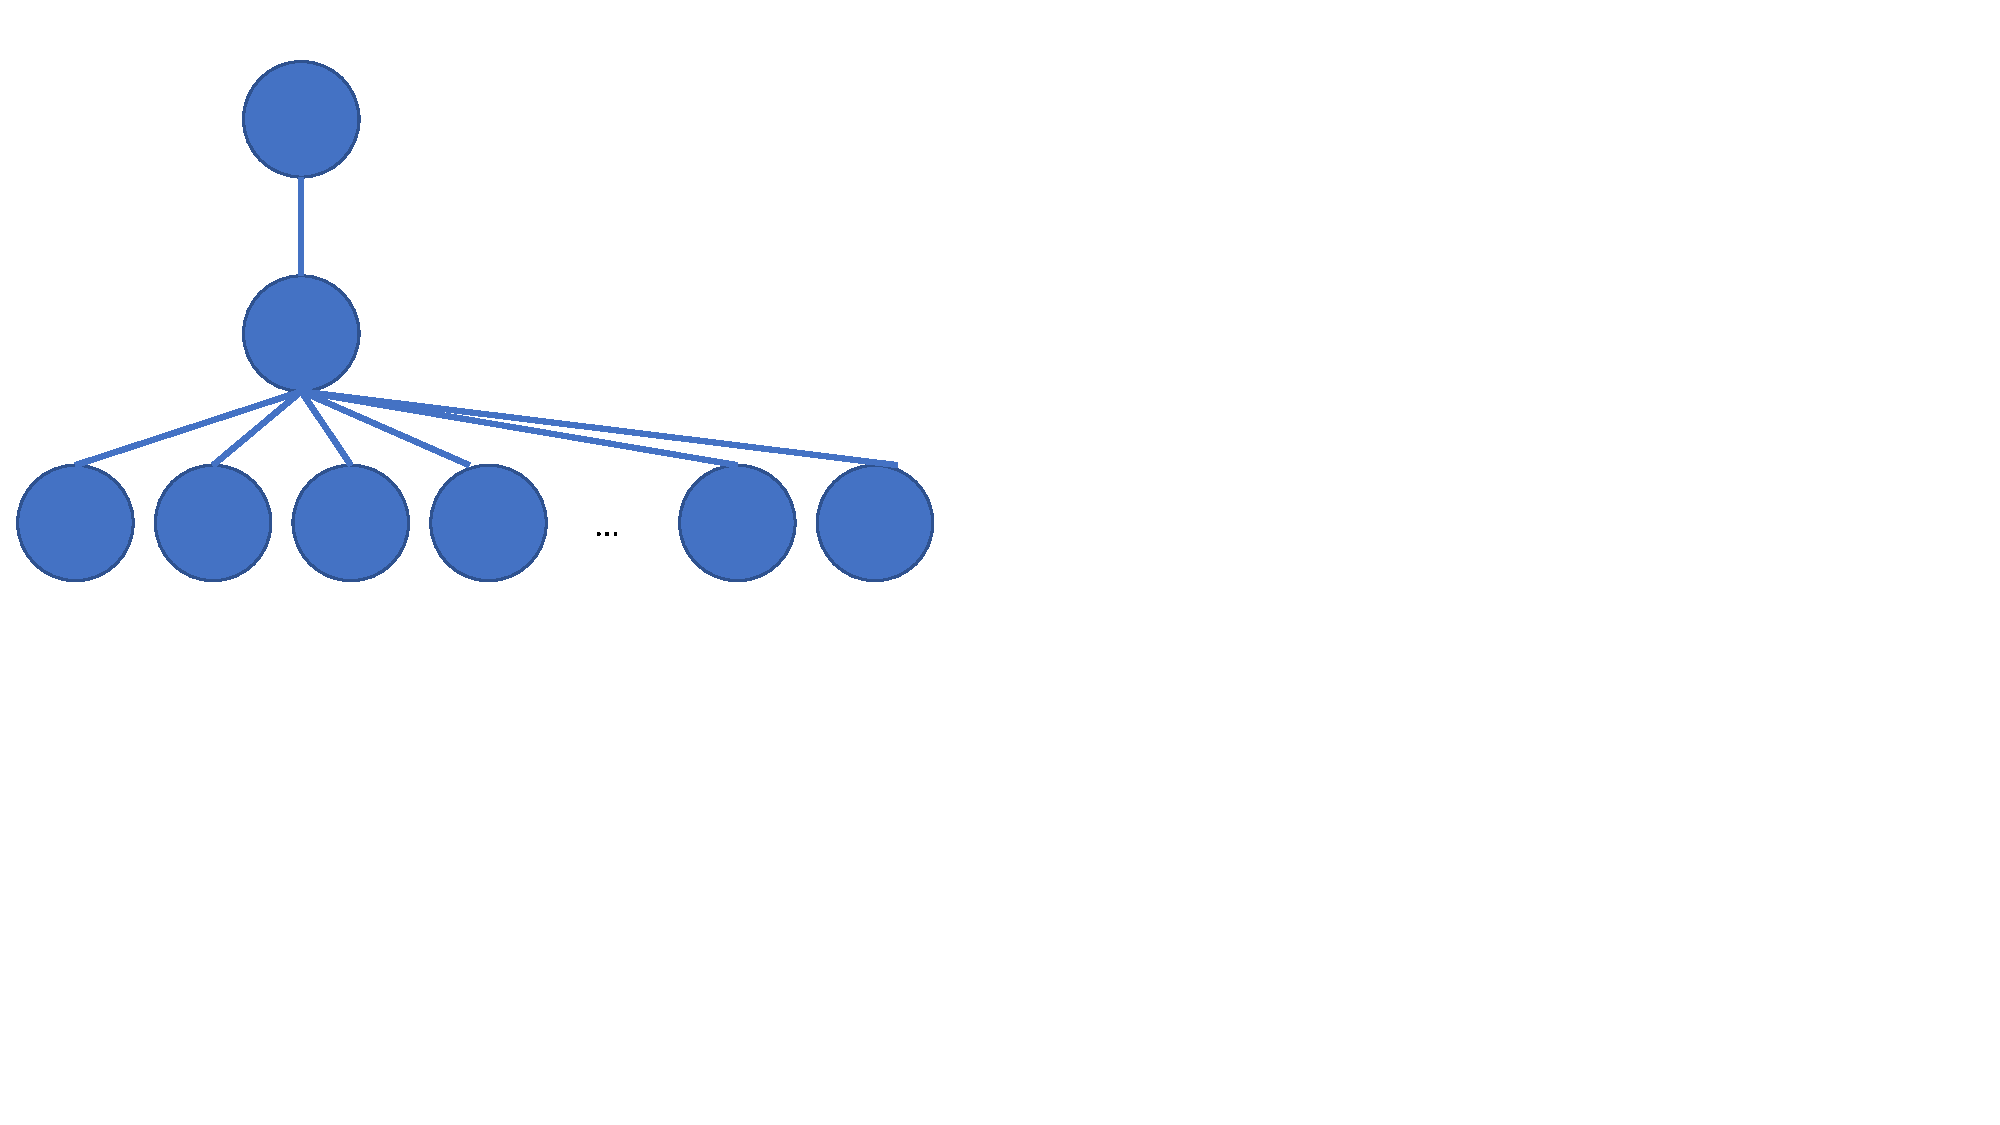
\includegraphics[width=0.4\textwidth,trim={0cm 7cm 18cm 0},clip]{figures/pipeline1.pdf}
\end{figure}
\end{frame}

\subsection{GHS [GHS86]}
\begin{frame}
\frametitle{GHS Algorithm}
\begin{itemize}
    \item A distributed version of \textbf{Boruvka's} algorithm: merging components.
    \item Each node starts as \textbf{a tree} with height 0.
    \item At phase $i$, any component with size less than $2^i$ fuses into another.
    \item Minimum outgoing edge (MWOE) of each component for merging.
    \item Worst case $O(n)$ rounds: the component can grow to size $O(n)$.
    \item $\log n$ phases, $O(n \log n)$ rounds.
\end{itemize}

\begin{figure}
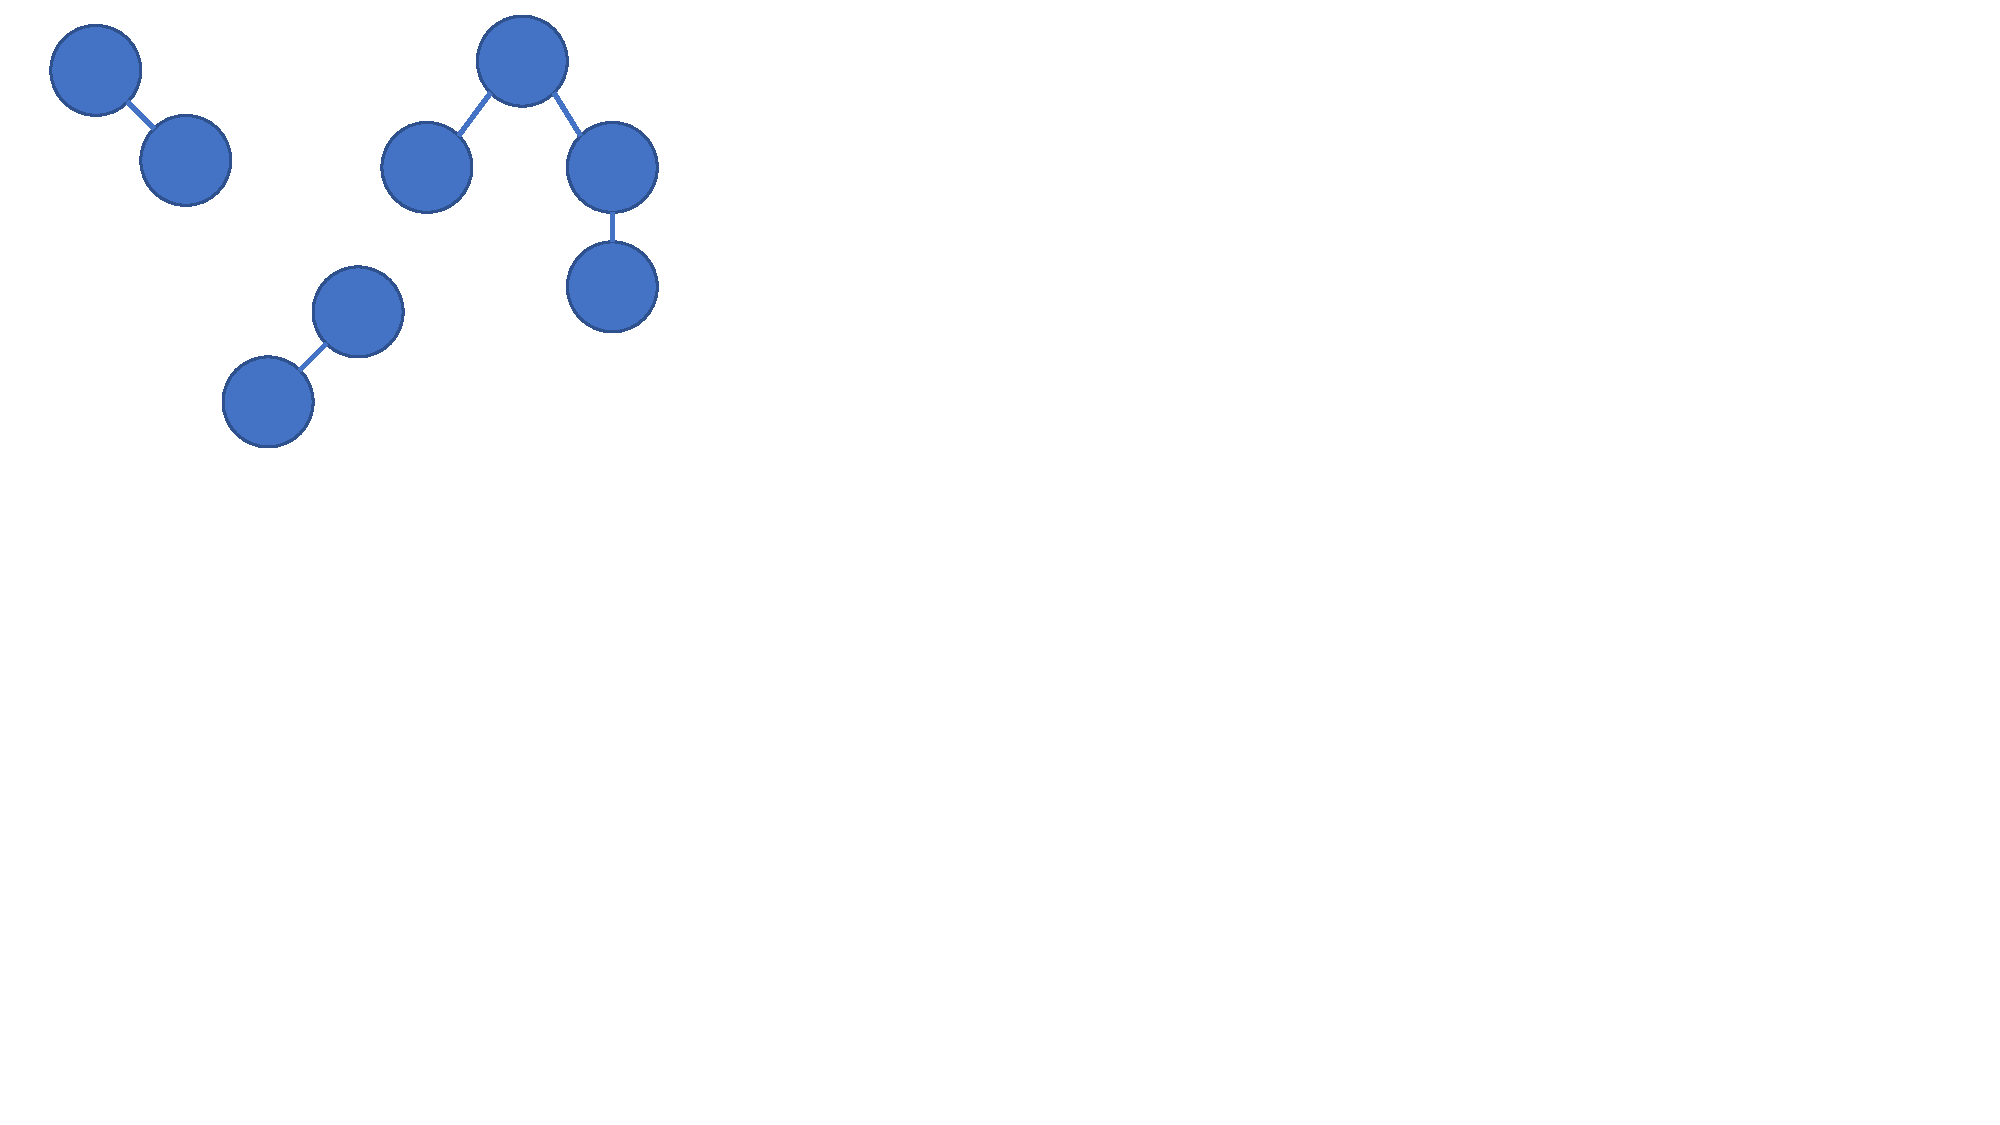
\includegraphics[width=0.4\textwidth,trim={0cm 10cm 18cm 0},clip]{figures/boruv1.pdf}
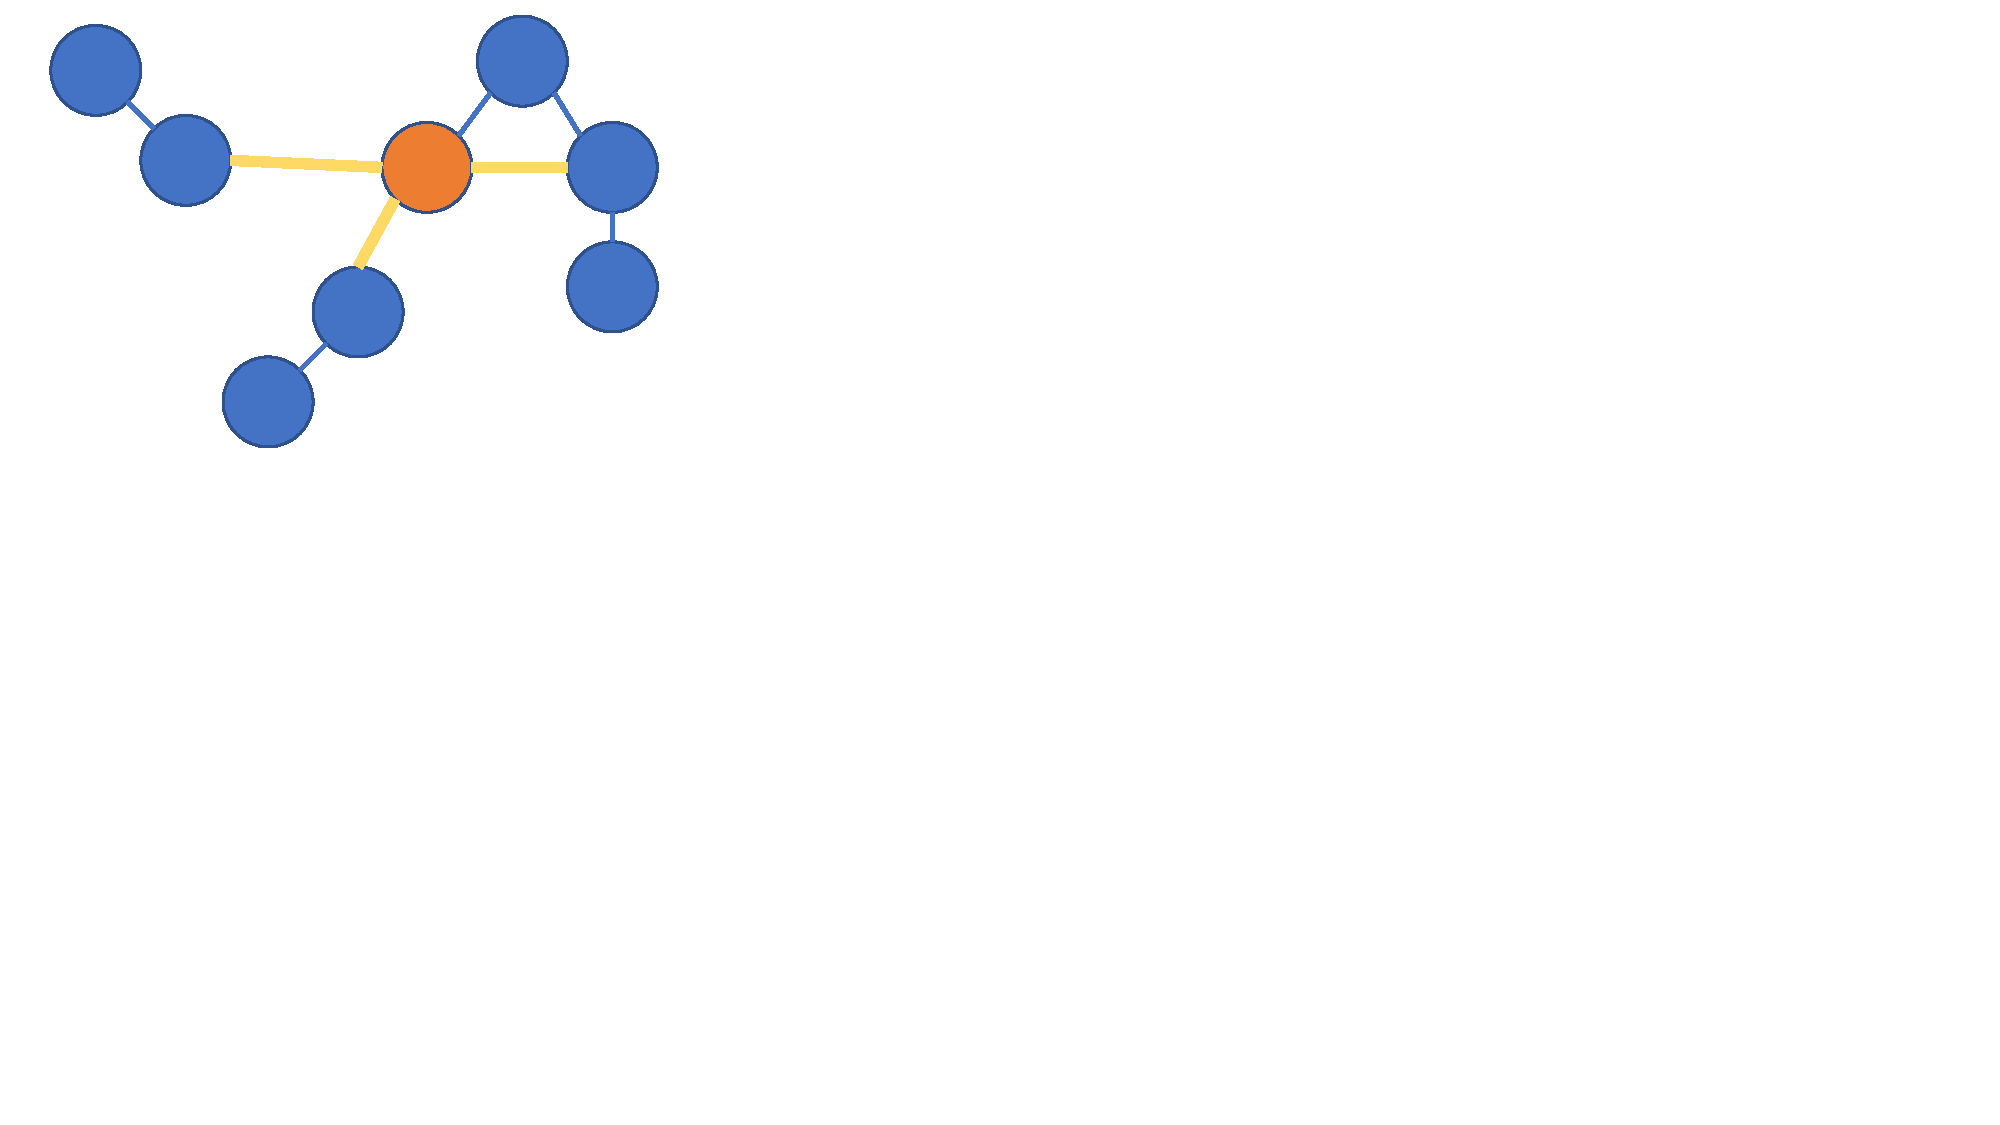
\includegraphics[width=0.4\textwidth,trim={0cm 10cm 18cm 0},clip]{figures/boruv2.pdf}
\end{figure}
\end{frame}

\begin{frame}
\frametitle{GHS Algorithm}
\begin{itemize}
    \item Each edge can only be accepted or declined once $O(m)$.
    \item Every round, each node needs to send convergecast and broadcast once, $O(n \log n)$.
    and $O(m + n \log n)$ messages.
\end{itemize}
\end{frame}

\subsection{Controlled-GHS [GKP98, KP98]}
\begin{frame}
\frametitle{Controlled-GHS Algorithm [GKP98, KP98]}
\begin{itemize}
    \item \textbf{Pipeline-MST} reduces 1 component every round: \textbf{slow}.
    \item \textbf{GHS} reduces the number of components by half, but \textbf{hard to merge giant components}.
    \item Why not combine the two algorithms?
\end{itemize}
\end{frame}

\begin{frame}
\frametitle{Controlled-GHS Algorithm [GKP98, KP98]}
\begin{itemize}
    \item Idea: \textbf{maximal matching} can bound the component size.
    \item Fact: \textbf{maximal matching} on rooted tree: $\log^*(n)$ rounds.
    \item In the first part, use \textbf{GHS} to reduce \# components to $\sqrt{n}$.
    \item In the second part, use \textbf{Pipeline-MST} for $O(D + \sqrt{n})$ rounds.
\end{itemize}
\begin{figure}
\centering
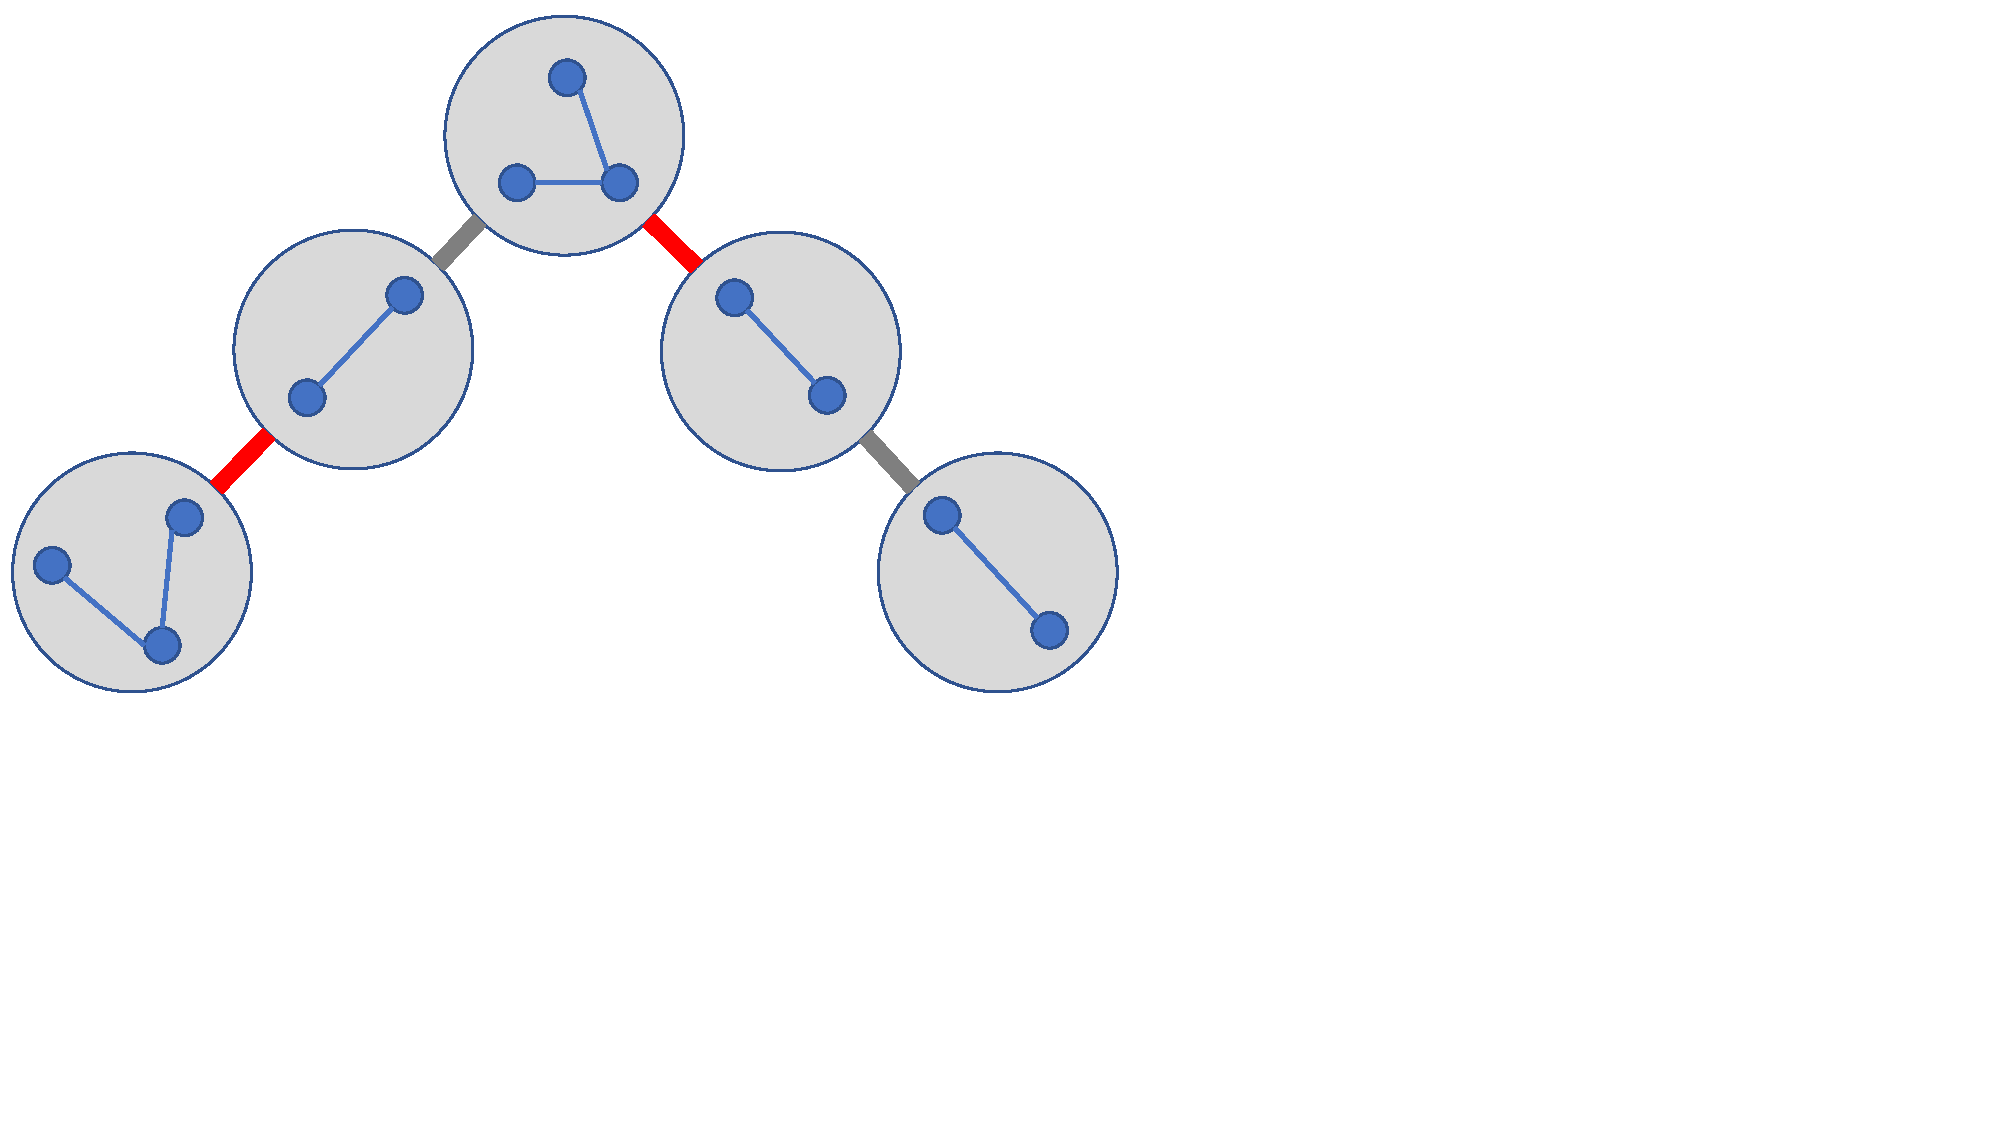
\includegraphics[width=0.4\textwidth,trim={0cm 5cm 12cm 0},clip]{figures/comptree.pdf}
\end{figure}
\end{frame}

\begin{frame}
\frametitle{Controlled-GHS Algorithm [GKP98, KP98]}
\begin{itemize}
\item $\log \sqrt{n}$ phases in the first part.
\item In each phase $i$, compute the maximal matching each component.
\item $O(2^i \log^*n)$ rounds (messages need to traverse at node level).
\item $O(2^i)$ rounds to broadcast within the component.
\item First part: $\sum_{i=0}^{\log \sqrt{n}} O(2^i \log^* n) = O(\sqrt{n}\log^*n)$ rounds.
\end{itemize}
\begin{figure}
\centering
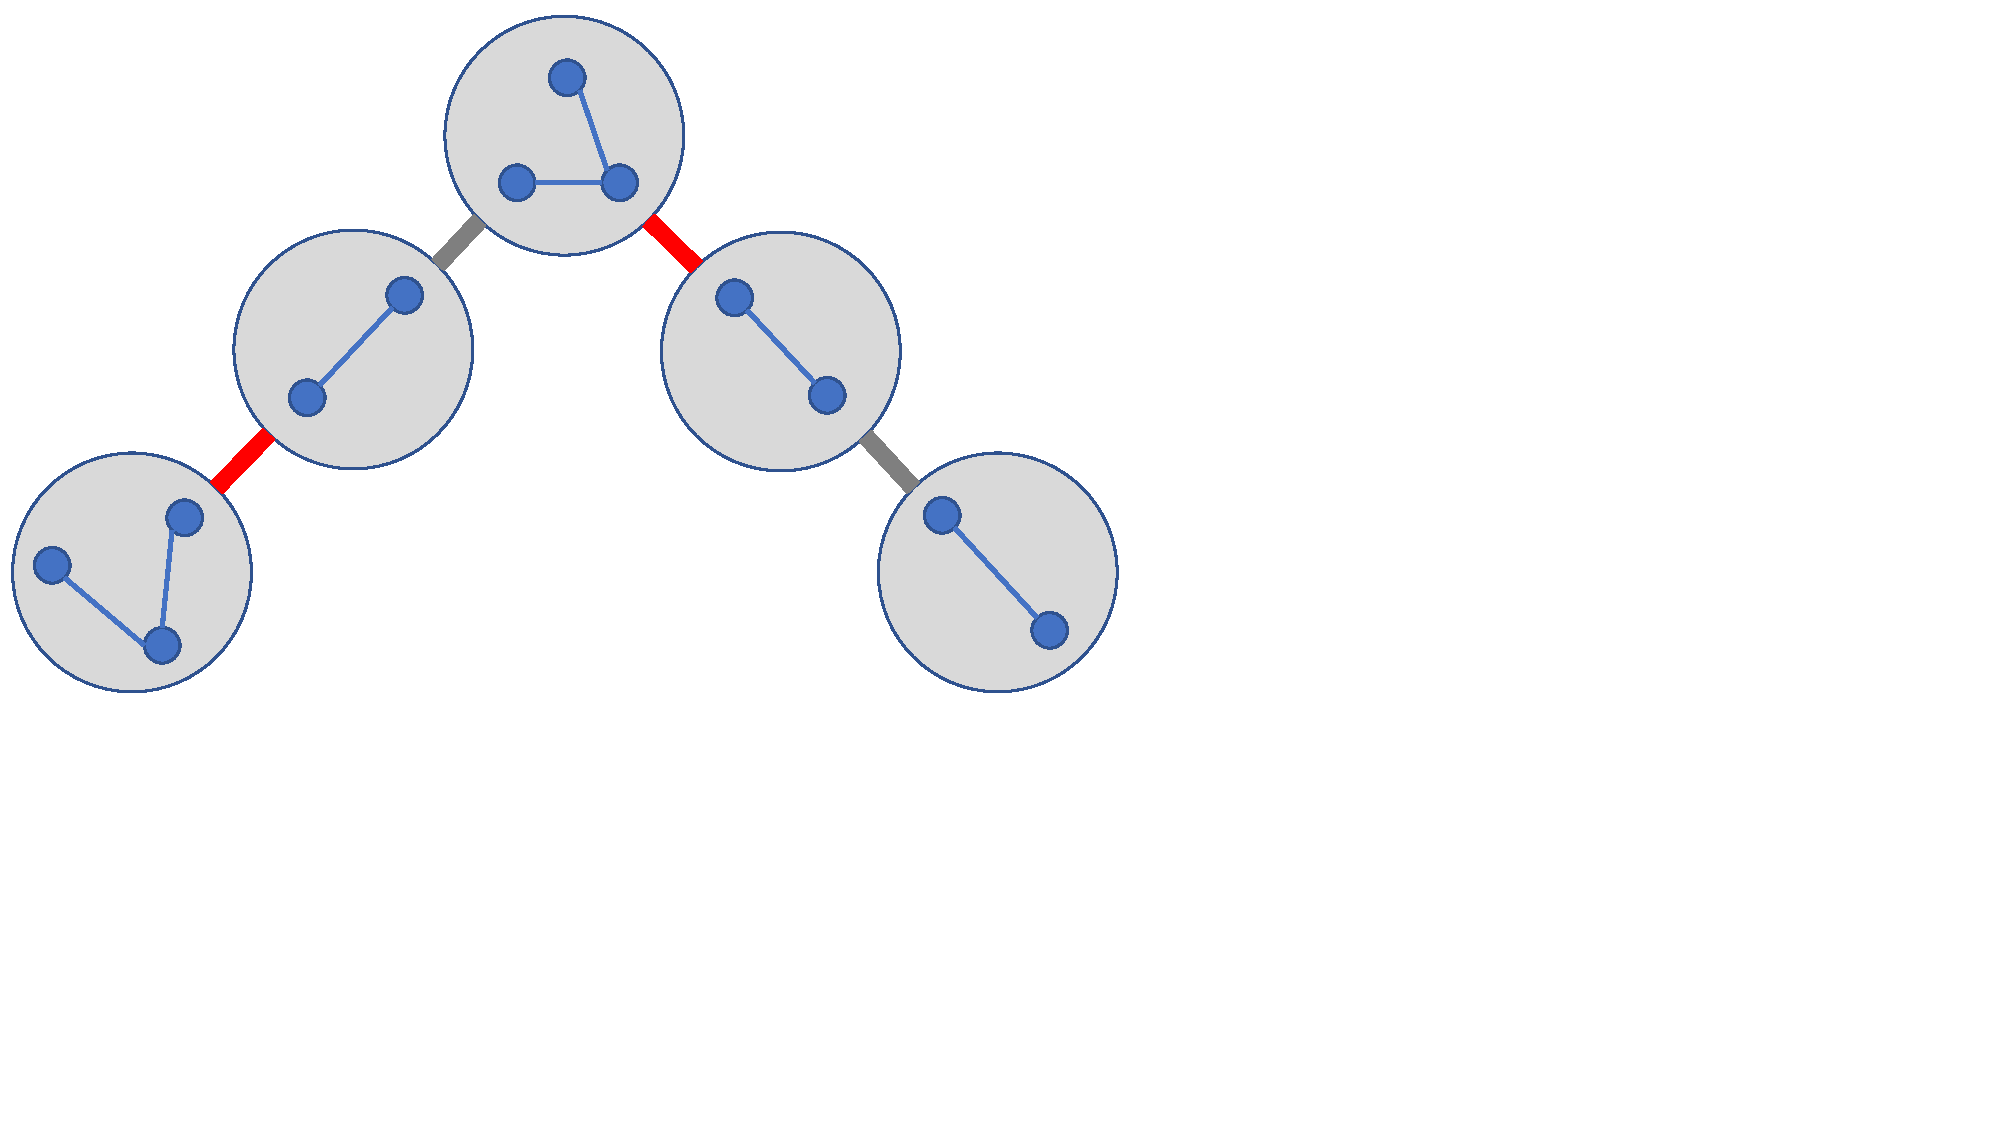
\includegraphics[width=0.4\textwidth,trim={0cm 5cm 12cm 0},clip]{figures/comptree.pdf}
\end{figure}
\end{frame}

\begin{frame}
\frametitle{Controlled-GHS Algorithm [GKP98, KP98]}
\begin{itemize}
\item Second part: Pipeline-MST, $O(D + \sqrt{n})$ rounds.
\item $O(D + \sqrt{n}\log^* n)$ rounds in total - \textbf{time-optimal}.
\end{itemize}
\end{frame}

\begin{frame}
\frametitle{Controlled-GHS Algorithm [GKP98, KP98]}
\begin{itemize}
\item \textbf{High} message complexity.
\item First part: $\log \sqrt n$ rounds. 
\item $O(m + n \log \sqrt{n}) = O(m + n\log n)$ messages.
\item Second part, $O(m)$ messages to build a BFS tree.
\item Each node sends $O(\sqrt{n})$ edges. 
\item Total message complexity: $O(m+n^{\frac{3}{2}})$ - \textbf{not optimal}.
\end{itemize}
\end{frame}